\documentclass[letterpaper]{article}
\usepackage{alifeconf}
\usepackage[utf8]{inputenc}
\usepackage{hyperref,mathtools,listings,color}
\usepackage[ngerman]{babel}
\graphicspath{{images/}}

\definecolor{black}{rgb}{0.0,0.0,0.0}
\definecolor{materialGrey}{rgb}{0.27,0.27,0.27}
\definecolor{materialGreen}{rgb}{0.0, 0.8, 0.6}
\definecolor{materialRed}{rgb}{0.82, 0.1, 0.26}
\definecolor{materialYellow}{rgb}{1.0, 0.5, 0.0}
\definecolor{materialBlue}{rgb}{0.0, 0.5, 1.0}
\definecolor{lightgray}{rgb}{.9,.9,.9}
\definecolor{gray}{rgb}{.5,.5,.5}
\definecolor{darkgray}{rgb}{.3,.3,.3}
\definecolor{purple}{rgb}{0.65, 0.12, 0.82}

 % document styles for listings
  \lstset{
    backgroundcolor=\color{white},
    basicstyle=\footnotesize\ttfamily,
    breakatwhitespace=true,
    breaklines=true,
    numbers=left,
    numbersep=5pt,
    deletekeywords={event}, 
    numberstyle=\tiny,
    showspaces=false,
    showtabs=false,
    language=html,
    keywordstyle=\bfseries\color{materialRed},
    commentstyle=\itshape\color{materialGreen},
    columns=fullflexible,
    xleftmargin=0.5cm,
    xrightmargin=1cm,
    frame=lr,
    framesep=8pt,
    framerule=0pt
  }

\lstdefinelanguage{JavaScript}{
  keywords={typeof, new, true, false, catch, function, return, null, catch, switch, var, if, in, while, do, else, case, break, length},
  keywordstyle=\color{materialBlue}\bfseries,
  ndkeywords={class, export, boolean, throw, implements, import, this},
  ndkeywordstyle=\color{darkgray}\bfseries,
  identifierstyle=\color{black},
  sensitive=false,
  comment=[l]{//},
  morecomment=[s]{/*}{*/},
  commentstyle=\color{purple}\ttfamily,
  stringstyle=\color{black}\ttfamily,
  morestring=[b]',
  morestring=[b]"
}

\lstset{
   language=JavaScript,
   backgroundcolor=\color{white},
   extendedchars=true,
   basicstyle=\footnotesize\ttfamily,
   showstringspaces=false,
   showspaces=false,
   stepnumber=0,
   numbers=left,
   numberstyle=\tiny\color{gray},
   numbersep=9pt,
   tabsize=2,
   breaklines=true,
   showtabs=false,
   captionpos=b
}
\lstset{literate=%
   *{0}{{{\color{materialYellow}0}}}1
    {1}{{{\color{materialYellow}1}}}1
    {2}{{{\color{materialYellow}2}}}1
    {3}{{{\color{materialYellow}3}}}1
    {4}{{{\color{materialYellow}4}}}1
    {5}{{{\color{materialYellow}5}}}1
    {6}{{{\color{materialYellow}6}}}1
    {7}{{{\color{materialYellow}7}}}1
    {8}{{{\color{materialYellow}8}}}1
    {9}{{{\color{materialYellow}9}}}1
}


\title{A ship routing algorithm and it's map visualization}
\author{Andreas Lorer$^{1}$ \and  Kevin Klugmann$^{1}$\\
\mbox{}\\
$^{1}$ Hochschule Ravensburg-Weingarten, Doggenriedstr. 88250 Weingarten \\
contact@andreaslorer.de, kevin.klugmann@gmail.com}


\begin{document}
\maketitle

\begin{abstract}
	In dieser Arbeit soll aufgezeigt werden, wie eine automatisierte Visualisierung von Kreuzschifffahrtsrouten realisiert werden konnte. Da das Meer eine offene Fläche ohne Begrenzungen darstellt, ergeben sich zahlreiche Probleme für eine Routenfindung. In unserem Ansatz erfolgt das Routing Grid-basiert auf einem HTML5-Canvas. Mittels diesem Grid soll die Route über eine variable Anzahl an Hafenpunkten durch Verwendung des A*-Algorithmus gefunden werden. Es stellte sich heraus, dass eine voll automatische Kartenvisualisierung möglich ist, welche noch viel Potenzial für zukünftige Verbesserungen bietet.
\end{abstract}

\section{Introduction}
	Während es im Bereich des Nahverkehrs relativ einfach ist, eine Route zu berechnen\footnotemark und diese in einer interaktiven Karte zu visualisieren, gibt es zum jetzigen Zeitpunkt keine Möglichkeit, dies für Schiffsrouten zu tun. Abbildung \ref{fig:visualisierungsproblem} zeigt eine Visualisierung, wie sie momentan in einer Karte zum Einsatz kommt. 

	\footnotetext{Via Google-Maps, Bing-Maps oder weiteren Kartenanbieter}

	\begin{figure}[!htb]
		\begin{center}
		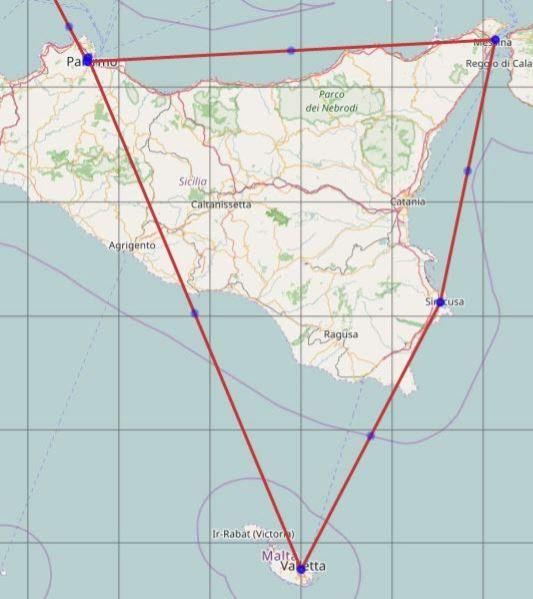
\includegraphics[width=2in]{visualisierungsproblem}
		\caption{Beispiel einer Kartenvisualisierung}
		\label{fig:visualisierungsproblem}
		\end{center}
	\end{figure}

	Die Grafik veranschaulicht bereits deutlich das zu lösende Problem: Die einzelnen Häfen sind nur durch gerade Linien verbunden, die nicht zwischen Wasser und Land unterscheiden. Dadurch führen Routen über Land. Für dieses Problem der automatischen Kartengenerierung wurde ein Algorithmus entwickelt, der in der Lage ist, zwischen Land und Wasser zu unterscheiden und damit eine visuell ansprechendere Visualisierung ermöglicht. Als Eingabe benötigt der Algorithmus eine Liste an Hafen-Positionen, aus welchen er eine Route generiert. Eingabe und Ausgabe werden dabei im \texttt{geojson-Format} \cite{rfc7946} eingelesen, beziehungsweise ausgegeben.

	Momentan werden Routen für die Kreuzschifffahrt vorwiegend auf zwei Arten visualisiert.

	\begin{figure}[!htb]
		\begin{center}
		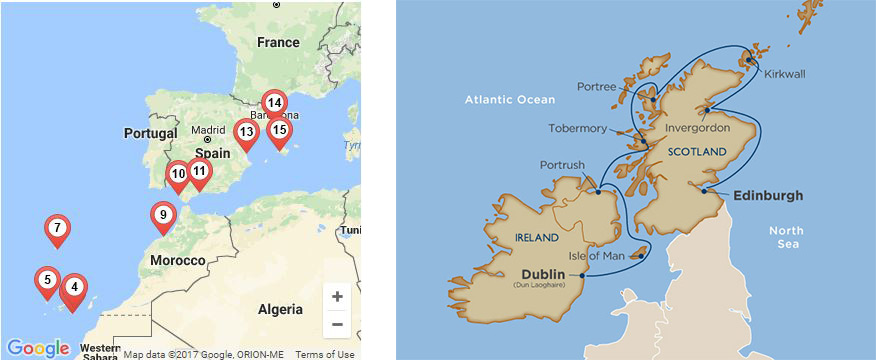
\includegraphics[width=\linewidth]{state_of_the_art}
		\caption{State of the art}
		\label{fig:state of the art}
		\end{center}
	\end{figure}

	Wie in Abbildung \ref{fig:state of the art} zu sehen ist, werden entweder nur einzelne Pin's auf die jeweiligen Häfen gesetzt oder es werden komplexe Vektorgrafiken händisch erzeugt. Letzteres ist sehr aufwändig und dementsprechend kostenintensiv. Einzig \url{http://www.cleancruising.com.au/} hatte eine visuell überzeugende Karte (Abbildung \ref{fig:state of the art cleancruise}) mit einem ansprechendem Routing. 

	\begin{figure}[!htb]
		\begin{center}
		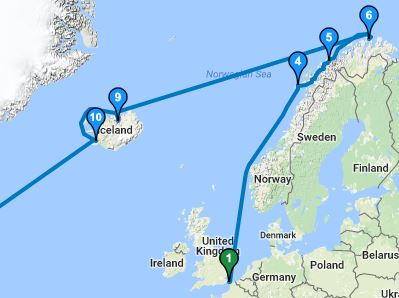
\includegraphics[width=.6\linewidth]{state_of_the_art_cleancruise}
		\caption{Kartenvisualisierung von cleancruise.com}
		\label{fig:state of the art cleancruise}
		\end{center}
	\end{figure}

	Entscheidend ist in unserem Fall nicht wie im klassischen Sinne die Berechnung des kürzesten Weges, sondern eine ästhetische Darstellung der Fahrtroute. Bei der Zielgruppe handelt es sich um Personen, die mittels eines Buchungsportals eine Kreuzfahrt buchen möchten. Ihnen soll die ungefähre Fahrtroute optisch ansprechend präsentiert werden. Die Route hat also keinerlei Relevanz für Nautiker oder Kapitäne. Wassertiefe oder nicht befahrbare Abschnitte sind deshalb irrelevant und werden von uns nicht beachtet. 

	Andere Bedingungen für einen Algorithmus sind oftmals seine lineare Laufzeit $O(n)$, die für Echtzeitsysteme benötigt werden. Unser Algorithmus ist allerdings nur für den Einsatz im Backend vorhergesehen. Dort werden die Routen für die Anzeige im Frontend bereits vorberechnet und zur Wiederverwendung abgespeichert. Eine lineare Laufzeit ist dadurch nicht von Nöten und war zu keiner Zeit eine Anforderung.

\section{Related Work}
	Es finden sich bisher nur wenige Publikationen, die sich mit dem Thema Schiffsrouten via Web-Plattform auseinandersetzen.\\

	Die meisten Systeme, die Routenberechnungen für die Schifffahrt durchführen, benutzen eine Graph basierte Grid-Struktur oder eine Abwandlung davon. \cite{makrygiorgos15} entwickelte beispielsweise eine \texttt{Novel Grid Structur} (siehe Abbildung \ref{fig:novel grid structure}). In dieser Datenstruktur werden für jeden Knotenpunkt (Node) maritime Informationen abgespeichert und Gewichtungen für jede Kante (Edge) berechnet.

	\begin{figure}[!htbp]
		\centering
		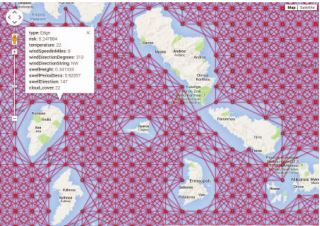
\includegraphics[width=.8\linewidth]{novel_grid_structure}
		\caption{Novel Grid Structure (Abbildung von \cite{makrygiorgos15})}
		\label{fig:novel grid structure}
	\end{figure}

	Die Motivation dahinter ist dabei meist ein Echtzeitsystem oder eine Echtzeitkalkulation der Route. Eine Grid-Struktur, die wie ein Graph aufgebaut ist, beschleunigt den Suchprozess des A*-Algorithmus erheblich\cite{patel16}. Die Grid-Struktur wird dabei aus den statischen maritimen Informationen und zusätzlichen dynamischen Daten (meterologische Wetterdaten über Windstärke, Windrichtung etc) für die Routenberechnung ergänzt \cite[s. 2]{makrygiorgos15}.
	Für unseren Algorithmus wäre es zwar hilfreich gewesen, eine solche Datenstruktur zu haben, allerdings verfügten wir über keinerlei Zugriff auf solche Datenquellen, da diese unseren Recherchen nach nicht öffentlich verfügbar sind.

\section{Die Pixel-Karte}
	In diesem Abschnitt möchten wir unsere Arbeit an dem Routing Algorithmus für Kreuzschifffahrten genauer erklären und den Problemlöseprozess aufzeigen. Unsere Lösung basiert zunächst auf der Generierung einer Pixel-Karte. Diese Karte dient uns als Grundlage für das Routing mittels A*-Algorithmus. Die Pixel-Karte aus Abbildung \ref{fig:Pixel Map Miami} wird durch Kartendaten von Natural Earth\footnotemark auf einem HTML5-Canvas erzeugt. 

	\footnotetext{Natural Earth 1:10m coastline \url{http://bit.ly/2kbyYIV}}

	\begin{figure}[!htbp]
		\centering
		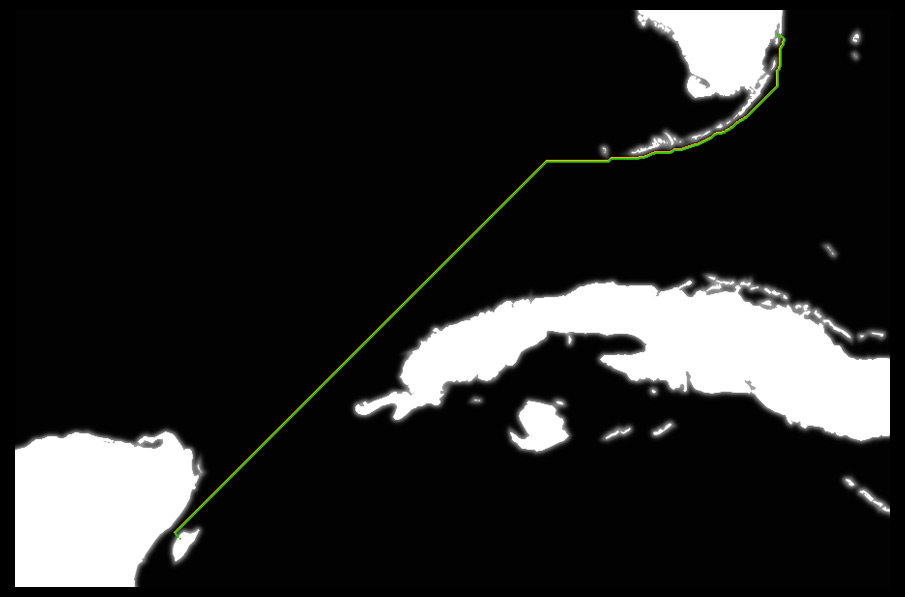
\includegraphics[width=\linewidth]{pixel_map_miami}
		\caption{Generierte Pixel-karte für eine Routenberechnung}
		\label{fig:Pixel Map Miami}
	\end{figure}

	Der Maßstab der Karte beträgt dabei 1:10m (Millionen) und liegt im Datenformat \texttt{.shp} (für Shapefile) vor. Diese wurde mittels eines Tools (QGIS) in \texttt{geojson} umgewandelt. Höher aufgelöstes Kartenmaterial ist im Netz an verschiedenen Stellen zu finden\footnotemark, haben allerdings Dateigrößen von bis zu 500 MB. Da wir solch hohe Datenmengen client-seitig nicht verarbeiten konnten, ist für uns die Karte mit dem Maßstab 1:10m ein solider Kompromiss zwischen nötiger Genauigkeit entlang der Küstenlinie (Inseln \& Fjorde etc.) und Datengröße.

	\footnotetext{z.B. bei OpenStreetMap \url{http://openstreetmapdata.com/data/coast}}

	Nachdem die Pixel-Karte auf dem Canvas gezeichnet ist, dient uns die Canvas-Auflösung als Grid-Raster. Höhere Auflösungen ermöglichen es dabei, mehr Details darzustellen. Das ist besonders für Fjorde und Inseln nötig, da diese bei einer zu niedrig aufgelösten Pixel-Karte nicht dargestellt werden können. Eine Auflösung von $512^2$ oder $1024^2$ wurde bei unseren Routenkalkulationen als ein solider Wert befunden und erzeugte gute Ergebnisse. Je höher die gewählte Auflösung, umso mehr Arbeitsspeicher wird allerdings auch benötigt. Da wir client-seitig eine Limitierung des verfügbaren Arbeitsspeichers durch den Browser haben, konnten höhere Kartenauflösungen nicht getestet werden. Sobald eine Portierung auf eine server-seitige Lösung via Node.js erfolgt, sollte dies allerdings möglich sein.

	\subsection{Pixel-Karte in Graustufen}
		Der HTML5 Canvas bietet die Möglichkeit, die Farbinformationen für jeden Pixel auszulesen. Ein schwarzer Pixel bedeutet dabei, dass es sich um Wasser handelt und ein weißer Pixel steht folglich für Land, also ein Hindernis. Wird jedoch lediglich zwischen Land und Wasser unterschieden, führt dies zu einem Problem: Die Schiffe fahren genau entlang der Küstenlinie, da dies dem kürzesten Weg von A nach B entspricht (siehe Abbildung \ref{fig:route before blur}).

		\begin{figure}[!htbp]
			\centering
			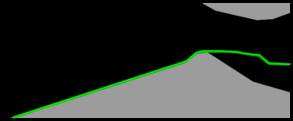
\includegraphics[width=.7\linewidth]{route_before_blur}
			\caption[]{Pixel Karte vor dem Blur-Effekt.\footnotemark}
			\label{fig:route before blur}
		\end{figure}
		\footnotetext{Das Land wurde ausgegraut, um die Route besser sichtbar zu machen}

		Da Schiffe allerdings nicht genau auf der Küstenlinie, sondern nur in Küstennähe fahren, würde dies den Vorstellungen von einer ästhetischen und möglichst realistischen Darstellung widersprechen. 

		Um dieses Problem zu lösen und eine glaubhaftere Schiffsroute zu generieren, musste die berechnete Route von der Küstenlinie versetzt werden. Dazu haben wir die Pixel-Karte in zwei Schritten einer Manipulation unterzogen, welche in Abbildung \ref{fig:blur effect} zu sehen ist.  Erstens wurde die Pixel-Karte 3 mal gezeichnet und dabei die Pinselgröße des Canvas jedes mal verringert (auf 6, 3, 0.1). Bevor dann in der letzten Iteration das Land gezeichnet wurde, erfolgte noch ein Gaussian Blur Filter\cite{vigour17}. Dieser bewirkt, dass die sehr harten Kanten, die beim Zeichnen entstehen, geglättet werden und ein homogener Übergang erreicht wird.

		\begin{figure}[!htbp]
			\centering
			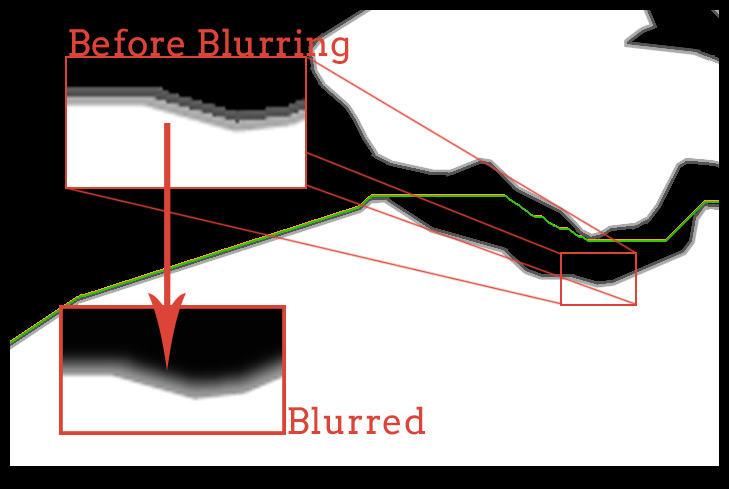
\includegraphics[width=\linewidth]{blur_effect}
			\caption{Anwendung eines Gaussian-Blur Filters}
			\label{fig:blur effect}
		\end{figure}

		Nach der Anwendung des Blur Filters wurde zuletzt die Landmasse eingezeichnet, damit diese ihre scharfe Kante behält und nicht durch den Blur in Unschärfe verschwimmt. 

		\subsection{A*-Kantengewichtung}
			Durch dieses Verfahren erhielten wir eine Pixel-Karte, die nicht nur Schwarz und Weiß, sondern auch Graustufen-Werte zwischen 0-255 beinhaltet. Der von uns verwendete A*-Algorithmus\cite{ginstead14} ermöglicht es, eine Kantengewichtung für die Routenberechnung mit einfließen zu lassen. Eine Kantengewichtung führt dazu, das gewisse Wege bevorzugt werden können. In unserem Fall hat die Farbe Schwarz die geringste Gewichtung und ist damit der absolut bevorzugte Weg, den der A*-Algorithmus wählen kann. Die Graustufen-Werte haben nun eine logarithmische Gewichtung die durch den RGB-Wert der Farbe errechnet wird.\\

			$weight = \lceil rgbValue * \ln{(rgbValue)/100} \rceil$\\

			Damit der A*-Algorithmus das Land nicht als Abkürzung verwendet, haben RGB-Werte über 250\footnotemark eine sehr viel höhere Gewichtung. Dadurch soll erreicht werden, dass das Land nur als aller letzte Möglichkeit überquert werden darf. Zum Beispiel dann, wenn die GPS Koordinate eines Hafens, innerhalb eines Kanals oder Flusses liegt, der im Kartenmaterial nicht enthalten ist. Deshalb erfolgt die Errechnung für RGB-Werte über 250 mittels der Gewichtung $weight = rgbValue^3$. Ein RGB Wert von 255 würde also eine Gewichtung von $255^3 = 16581375$ bedeuten. Wohingegen ein RGB Wert von beispielsweise 120 nur $ weight = \lceil 120 * ln(120)/100 \rceil = \lceil 5.774 \rceil = 6 $ ergeben würde. Die Gewichtung der Grauwerte zwischen 1-249, werden folglich auf einen Wertebereich von 1-14 gemappt.\\

			\footnotetext{Werte die schon sehr nahe an der Farbe Weiß liegen.}

			\begin{figure}[!htbp]
				\centering
				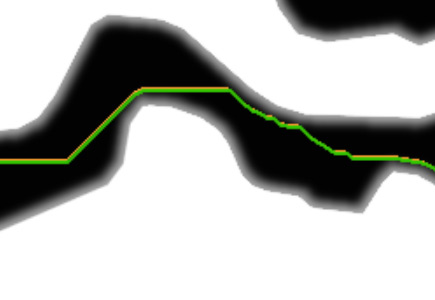
\includegraphics[width=0.7\linewidth]{route_after_blur}
				\caption{Ergebnis der Routenberechnung mit Blur Filter Pixel-Karte}
				\label{fig:route_after_blur}
			\end{figure}

			Wie in Abbildung \ref{fig:route_after_blur} zu sehen ist, beeinflusst nun die Gewichtung der RGB Werte die Wahl der eingeschlagenen Route. Dadurch wird die Route weg von der Küstenlinie "`geschoben"' und visualisiert nun zunehmend das reale Verhalten einer Schiffsroute.

\section{Verbesserung der routing Genauigkeit}
	Zuerst erfolgten unsere Berechnungen mithilfe einer einzigen Pixel-Karte. Dies funktionierte sehr gut, solange die einzelnen Häfen einer Route relativ nahe zusammen lagen.

	Für weitläufigere Routen war die Kartenauflösung jedoch zu grob, da sehr weit weg gezoomt werden musste, um alle Hafenpunkte auf der Karte zu erfassen.
	Um dieses Problem zu lösen, berechneten wir schließlich jeden Abschnitt einer Route einzeln. Bei einer Route über die Punkte A, B und C werden also die Routen AB und BC separat berechnet und dann für jeden Abschnitt eine eigene Pixel-Karte erzeugt.

	\begin{figure}[!htbp]
		\centering
		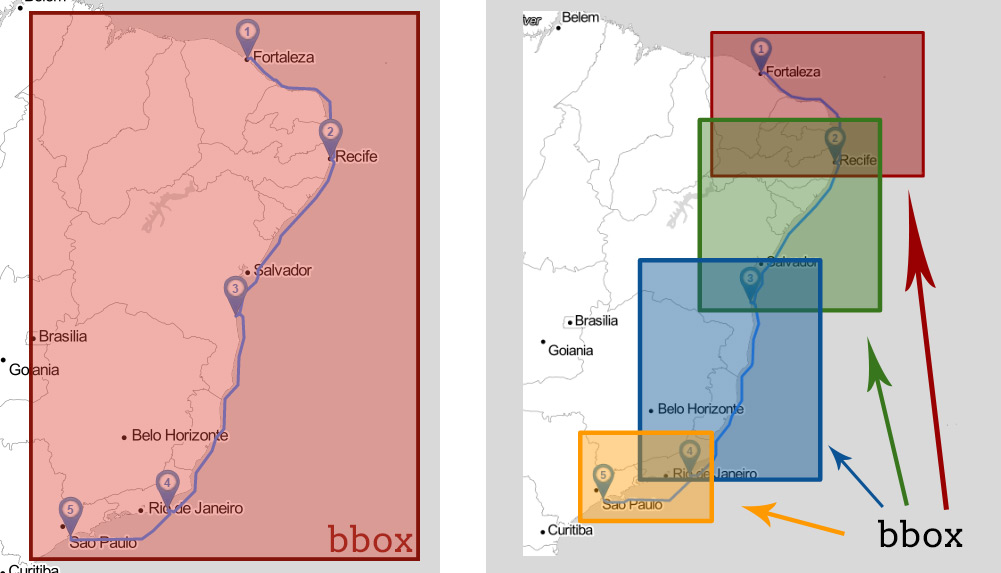
\includegraphics[width=\linewidth]{bbox_clipping}
		\caption{Unterteilung der Route in einzelne Abschnitte (rechts), anstatt wie zuvor, in einen einzelnen Abschnitt (links)}
		\label{fig:bbox_clipping}
	\end{figure}

	Um dies zu ermöglichen, wird für jeden Abschnitt eine \texttt{bbox} (Bounding Box) für den jeweiligen Routenabschnitt berechnet (siehe Abbildung \ref{fig:bbox_clipping}). Diese bbox wird dann nochmals ein wenig vergrößert, um einen Puffer zu haben und dient dann dem A*-Algorithmus für die Wegfindung.
	Dadurch wird erreicht, dass Routenabschnitte, die weiter von einander entfernt liegen, eine andere Zoomstufe besitzen als Routen, die näher zusammen verlaufen. Abbildung \ref{fig:bbox_clipping_pixelmap} zeigt zwei Pixel-Karten, die für eine Fahrtroute in Norwegen berechnet wurden. Wie zu sehen ist, weisen sie ganz unterschiedliche Zoom-Stufen auf, was eine Routenführung durch die Fjorde erst möglich macht.

	\begin{figure}[!htbp]
		\centering
		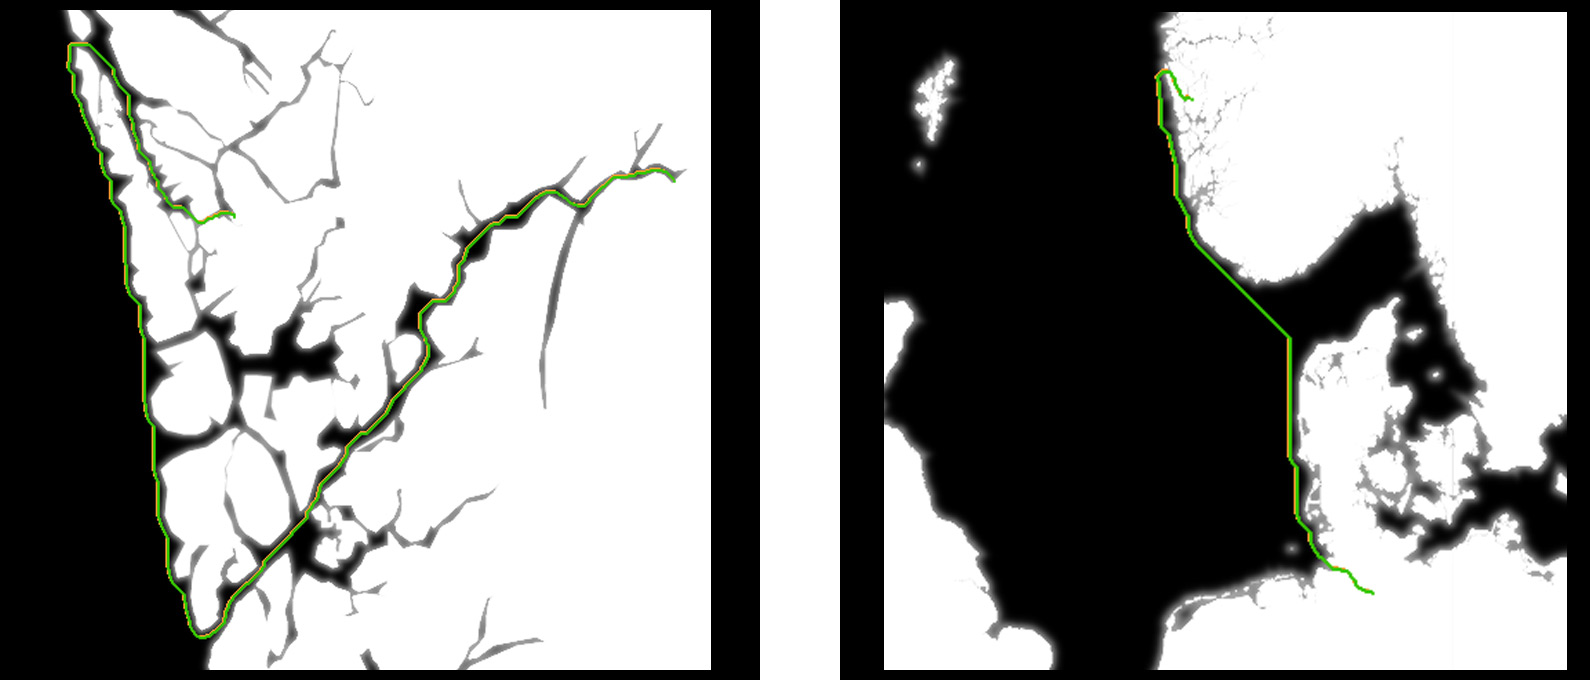
\includegraphics[width=\linewidth]{bbox_clipping_pixelmap}
		\caption{Zwei Beispiele für eine Pixel-Karte die für den jeweiligen Abschnitt unterschiedliche Zoom-Stufen aufweisen.}
		\label{fig:bbox_clipping_pixelmap}
	\end{figure}

\section{Karten Rasterisierung}
	Da das Kartenmaterial die ganze Erde umfasst, mussten Optimierungen gefunden werden, damit die Berechnungszeiten für unsere Route in einem akzeptablen Rahmen bleiben. Durchschnittlich haben wir Routen mit 6 Hafenpunkten, bei welchen die Berechnugszeit im Schnitt bei ~37sec liegt.\\

	In einem ersten Ansatz verfolgten wir das Ziel, die Polygone unseres Kartenmaterials auf die Größe der bbox zuzuschneiden. Dies führte zu allerlei Problemen, die nicht gelöst werden konnten. So hatte beispielsweise die Library zum Zuschneiden an sich schon einen für uns kritischen Fehler\footnotemark, sodass eine andere Lösung gefunden werden musste.
	\footnotetext{Stand 14.02.2017: \url{https://github.com/w8r/martinez/issues/11}}

	Der zweite Ansatz bestand darin, nur diejenigen \texttt{geojson-Features} auszuwählen, die für die jeweilige Routenberechnungen relevant sind (Abbildung \ref{fig:select_features}).

	\begin{figure}[!htbp]
		\centering
		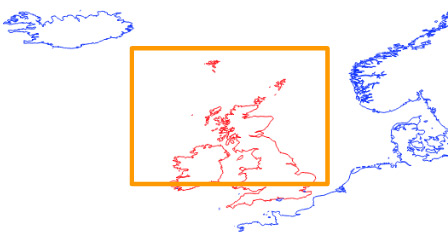
\includegraphics[width=\linewidth]{select_features}
		\caption{Auswahl der relevanten geojson-Features via bbox}
		\label{fig:select_features}
	\end{figure}

	Wie zu sehen ist, würde dies für eine Route in Großbritannien ganz passabel funktionieren. Abbildung \ref{fig:select_features_problem} zeigt allerdings, dass es Probleme gibt, sobald eine Route zum Beispiel nicht nur in Großbritannien, sondern auch in Bereiche benachbarter Staaten reichen würde. 

	\begin{figure}[!htbp]
		\centering
		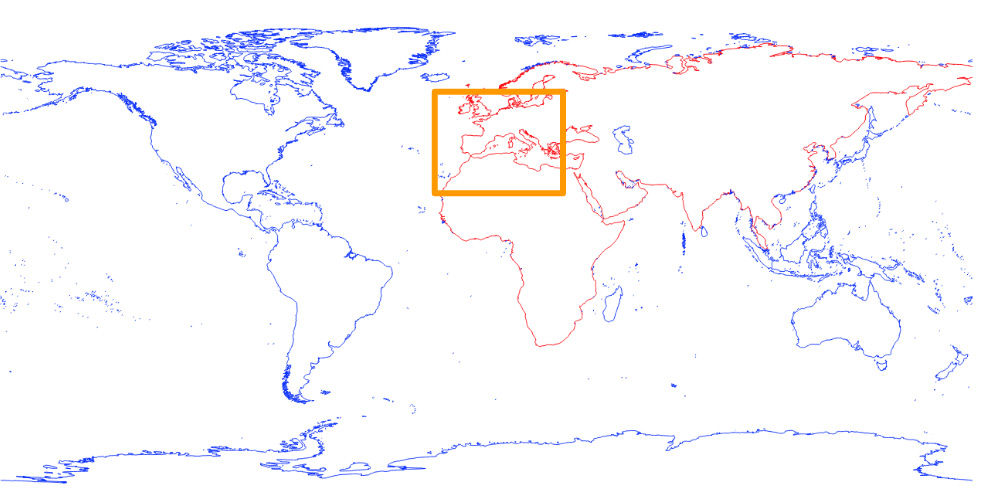
\includegraphics[width=\linewidth]{select_features_problem}
		\caption{Problematik wenn Auswahl nur über Features erfolgt}
		\label{fig:select_features_problem}
	\end{figure}

	Da unser Kartenmaterial aus der Küstenlinie besteht, ist das Feature für Europa gleichzeitig auch mit Asien, Afrika usw. verbunden, sodass es nicht möglich ist, einzelne Bereiche wie beispielsweise "`nur Deutschland und Dänemark"' zu selektieren. Dies hatte zur Folge, dass immer noch sehr lange Rechenzeiten benötigt wurden, da der \texttt{Overhead} nach wie vor enorm war. Abhängig von der Länge und der Position der Route wurden Rechenzeiten von bis zu einer Stunde benötigt.

	Infolgedessen haben wir das Kartenmaterial in einzelne Teile aufgeteilt.\footnote{Verwendet wurde dabei QGIS\cite{qgis}, zusammen mit dem \texttt{Grid-Splitter} Plugin.}

	\begin{figure}[!htb]
		\centering
		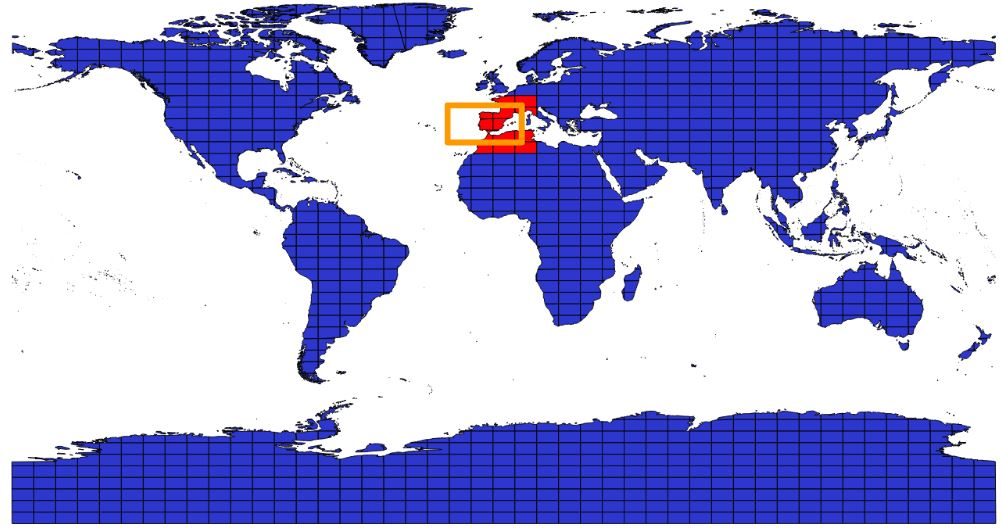
\includegraphics[width=\linewidth]{grid_splitter}
		\caption{Zerteilung der Karte in 2025 Tiles}
		\label{fig:grid_splitter}
	\end{figure}

	Dadurch sind wir in der Lage, nur noch diejenigen Polygone auszuwählen, die für unsere Route benötigt werden. Dadurch konnte das Berechnen der Pixel-Karte erheblich beschleunigt werden.

\section{Das Tool}
	Unser Tool, ist in Abbildung \ref{fig:tool} zu sehen und im Web erreichbar unter\footnotemark.

	\footnotetext{Ship-Routing Tool: \url{https://andi-lo.github.io/ship-cruising/dist/}}

	\begin{figure}[htbp]
		\centering
		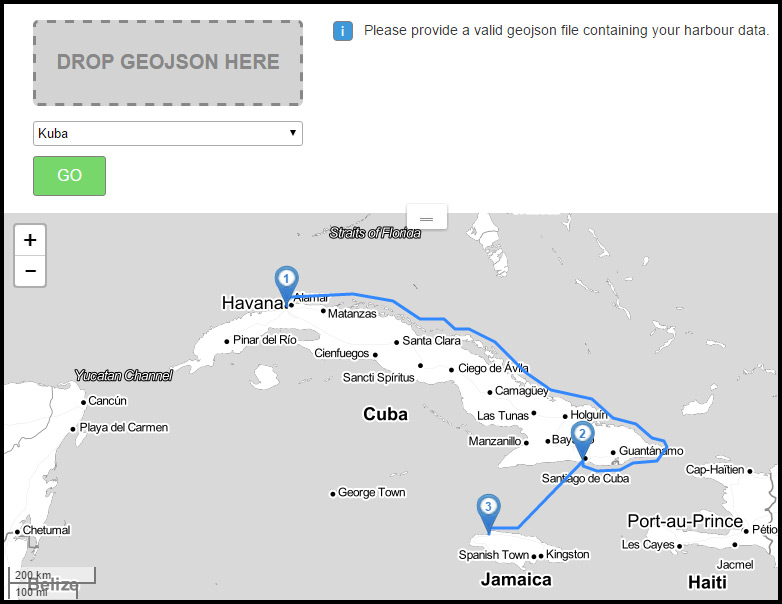
\includegraphics[width=\linewidth]{tool}
		\caption{User Interface unseres Tools}
		\label{fig:tool}
	\end{figure}

	Es besitzt ein interaktives Interface, das ein Dropdown-Menü zum Auswählen von vordefinierten Schiffsrouten und eine Drag \& Drop Funktionalität beinhaltet. 
	Mittels Drag \& Drop können valide\footnotemark geojson-Dateien zuerst hochgeladen und danach mittels "`Go-Button"' direkt die Route berechnet werden. Eine Route wird dabei als geojson-Objekt vom Typ \texttt{FeatureCollection<Point>} (siehe Anhang: Listing \ref{lst:geojson_example}) spezifiziert.
	Nachdem die Route berechnet wurde, wird sie in die Karte eingezeichnet und weitere Interaktionen wie z.B. Pinching oder Zoom sind möglich.

	\footnotetext{Eine Validierung der geojson-Datei auf Korrektheit erfolgt dabei nicht}

\section{Fazit}
	Es gibt mehrere Möglichkeiten, um sowohl unser Tool als auch das visuelle Ergebnis, weiter zu verbessern.

	\subsection{Schnellerer Suchalgorithmus}
		Für Anwendungen, die den A*-Algorithmus auf einer grid-basierten Struktur verwenden, gibt es verschiedene Optimierungsmöglichkeiten. Sowohl eine Änderung der Heuristic, als auch "`Map Preprocessing"'.

		Ein Beispiel: Wird ein Schritt nach Norden und dann nach Osten gegangen, dann ist dies meistens dasselbe, wie wenn  zuerst nach Osten und dann nach Norden gegangen wird. Graph-Algorithmen kennen allerdings weder "`Norden"' noch "`Osten"' und müssen deshalb beide Fälle ausprobieren.\cite[vgl.]{patel16} Dieses Verhalten nennt man "`Path Symmetries"'.

		\begin{quote}
			\textit{"`Two grid paths are symmetric if they share the same start and end point and one can be derived from the other by swapping the order of the constituent vectors."'}\cite[p. 1]{harabor12}
		\end{quote}

		In \cite{harabor12} wird der "`RSR-Algorithmus"' (Rectangular Symmetry Reduction) als Pathfinding Algorithmus beschrieben, der diese Symmetrien aufheben soll.\\

		\begin{quote}
			\textit{"`RSR can be described as a pre-processing algorithm which identifies symmetries by decomposing the grid map into empty rectangular regions."'}\cite[p. 2]{harabor12}\\

			\textit{"`[...] We observed that in most cases RSR can consistently speed up A* search by a factor of between 2-3 times (Baldur's Gate), 2-5 times (Adaptive Depth) and 5-9 times (Rooms). In some cases the gain can be much higher: up to 30 times."'}\cite[p. 4]{harabor12}
		\end{quote}

		Die wohl umfangreichste Javascript Pathfinding Library\footnotemark hat allerdings bis jetzt noch keine fertige RSR Implementierung. RSR ist in seiner ursprünglichen Form allerdings auch nur für einheitlich gewichtete Graphen verwendbar und es müsste eine Möglichkeit gefunden werden, RSR auf gewichtete Graphen zu übertragen. Dies wäre allerdings ein Forschungsfeld für sich.

		\footnotetext{Pathfinding.js:\url{https://github.com/qiao/PathFinding.js}}

	\subsection{Änderung der Heuristik}
		Der Sinn von einer Heuristik für den A*-Algorithmus ist es, eine Abschätzung für die Länge des kürzesten Pfads zu geben. Je besser die geschätzte Distanz dem kürztesten Pfad entspricht, umso schneller ist der A*-Algorithmus. Momentan wird eine Heuristik eingesetzt, die diagonale Bewegungen erlaubt. Die Heuristik könnte aber auf verschiedene Arten verbessert werden. In \cite{andrew04} wird ein Verfahren vorgestellt, bei dem die Grid-Map vor dem Pathfinding analysiert wird, um eine bessere Heuristik zu generieren.\\

		In "`A New Method of Ship Routing on Raster Grids, with Turn Penalties and Collision Avoidance"'\cite{szlapczynski06} wird die Heuristik dem Verhalten eines Schiffes angenähert. So sind Kursänderungen immer mit einem Verlust an Geschwindigkeit oder einer Verlängerung der Route verbunden. Dieses Verhalten wird nun auch durch die Heuristik wiedergespiegelt und Kursänderungen sind mit "`Kosten"' verbunden, sodass sie, wenn möglich, zu vermeiden sind. Dieses Verhalten könnte sich visuell auch positiv auf unseren Algorithmus auswirken, da momentan der von A* gefundene Weg sehr kantig verläuft.

	\subsection{Quad-Tree Preprocessing}
		Es wäre darüber hinaus auch möglich, die Pixel-Karte in quadratische Regionen zu unterteilen. Große, offene Flächen könnten damit durch nur wenige Quadrate repräsentiert werden und unregelmäßige Kanten entlang der Küste würden durch viele kleine Quadrate entstehen. Eine Implementierung ist zum Beispiel hier zu sehen: \url{https://www.youtube.com/watch?v=95aHGzzNCY8}. Weitere Optimierungsmöglichkeiten für den A*-Algorithmus sind unter \cite{patel16} zu finden.

	\subsection{Vorberechnung der Pixel-Karte}
		Um ein noch besseres Ergebnis zu erreichen, wäre es außerdem denkbar, einige Vorberechnungen zu tätigen. Anstatt die Pixel-Karte für jede Route neu zu berechnen und zu zeichnen, wäre es auch möglich, diese vorab einmalig zu errechnen. Die Auflösung müsste allerdings entsprechend hoch sein. Um die Effizienz zu steigern, könnte die gespeicherte Karte wiederum in Teile zerlegt werden. Dadurch könnte man bei einer Berechnung auf eine bereits vorliegende Karte zurückgreifen und sich hierbei die jeweiligen Berechnungskosten ersparen.

		Letztlich könnte es auch zielführend sein, das Kartenmaterial von den diversen  Kartenanbieter zu verwenden. Diese sind bereits für alle Zoomstufen vorhanden und sehr präzise. Was ihnen allerdings fehlen würde, wäre der "`Blur-Effekt"', den unsere Karte verwendet, um den Routenverlauf von der Küstenlinie zu verschieben.


{\footnotesize \bibliographystyle{acm}
\bibliography{references}}

\section{Anhang}
		Beispiel einer Route mit 3 Wegpunkten (Häfen) im \texttt{geojson-Format}

		\begin{lstlisting}[captionpos=b, caption=Beispiel Route: Kuba, label=lst:geojson_example, breaklines=false]
{
  "type": "FeatureCollection",
  "features": [
    {
      "type": "Feature",
      "properties": {},
      "geometry": {
        "type": "Point",
        "coordinates": [
          -82.36,
          23.14
        ]
      }
    },
    {
      "type": "Feature",
      "properties": {},
      "geometry": {
        "type": "Point",
        "coordinates": [
          -75.87,
          19.98
        ]
      }
    },
    {
      "type": "Feature",
      "properties": {},
      "geometry": {
        "type": "Point",
        "coordinates": [
          -77.93,
          18.46
        ]
      }
    }
  ]
}
		\end{lstlisting}

\end{document}
